\documentclass{protokol}
\usepackage[T1]{fontenc}
\usepackage{chemformula}

\leftheader{Studium atomových emisních spekter}
\centerheader{Praktikum IV}
\rightheader{Tomáš Derner}

\begin{document}

    \section*{Úkol}

    \begin{enumerate}

        \item S použitím spektra rtuti zkalibrujte hranolový spektrometr.
        Pro vyloučení hrubých chyb vyneste kalibrační křivku ihned do grafu.
        \item Ověřte vlnové délky sodíkových dubletů (alespoň tří).
        \item Na základě pozorování sodíkových dubletů diskutujte rozlišovací schopnost spektrometru.
        Diskutujte přesnost takto určené rozlišovací schopnosti.
        \item Prohlédněte si spektra výbojek s náplní \ch{He}, \ch{Ne}, \ch{Ar}, \ch{N2} a \ch{CO2}.
        Určete vlnové délky nejjasnějších čar.
        Porovnejte s tabulkovými hodnotami.
        \item Změřte vlnové délky čar \ch{H_{$\alpha$}}, \ch{H_{$\beta$}}, \ch{H_{$\gamma$}} Balmerovy serie vodíkového spektra.
        Vypočítejte Rydbergovu konstantu.

    \end{enumerate}

    \section*{Teorie}

    V této úloze studujeme atomová emisní spektra plynů.
    Využíváme k tomu hranolový spektrometr Hilgerova typu, jehož detailní popis je uveden ve studijním textu~\cite{pokyny}.
    Tento spektrometr neudává přímo vlnové délky pozorovaných čar, je proto potřeba jej okalibrovat pomocí známých vlnových délek emisního spektra rtuti.
    Tabulkové hodnoty těchto vlnových délek jsou uvedeny v sekci výsledků měření v tabulce~\ref{tab:kalibrace}.

    Pro rozlišovací schopnost $R$ spektrometru platí vztah
    \begin{equation} \label{eq:R}
        R = \frac{\lambda}{d\lambda},
    \end{equation}
    který určuje minimální rozdíl vlnových délek $\lambda$ a $\lambda + d\lambda$, který ještě spektrometr dokáže rozlišit.
    V tomto případě využijeme pro určení rozlišovací schopnosti měření dubletů sodíku.

    Ve viditelném emisním spektru vodíku jsou pozorovatelné čtyři čáry \ch{H_{$\alpha$}} (červená), \ch{H_{$\beta$}} (modrozelená), \ch{H_{$\gamma$}} (modrá) a \ch{H_{$\delta$}} (fialová).
    Tyto čáry jsou součástí tzv. Balmerovy série, pro vlnočty jejíž spektrálních čár platí vztah
    \begin{equation} \label{eq:rydberg}
        \sigma = \frac{1}{\lambda} = R \left( \frac{1}{4} - \frac{1}{n^2} \right),
    \end{equation}
    kde $R$ je Rydbergova konstanta a $n = 3, 4, 5, 6$ jsou přirozená čísla odpovídající jednotlivým čarám.
    Rydbergovu konstantu určíme z tohoto vztahu metodou nejmenších čtverců.



    \section*{Výsledky}

    \begin{figure}[h]
        \centering
        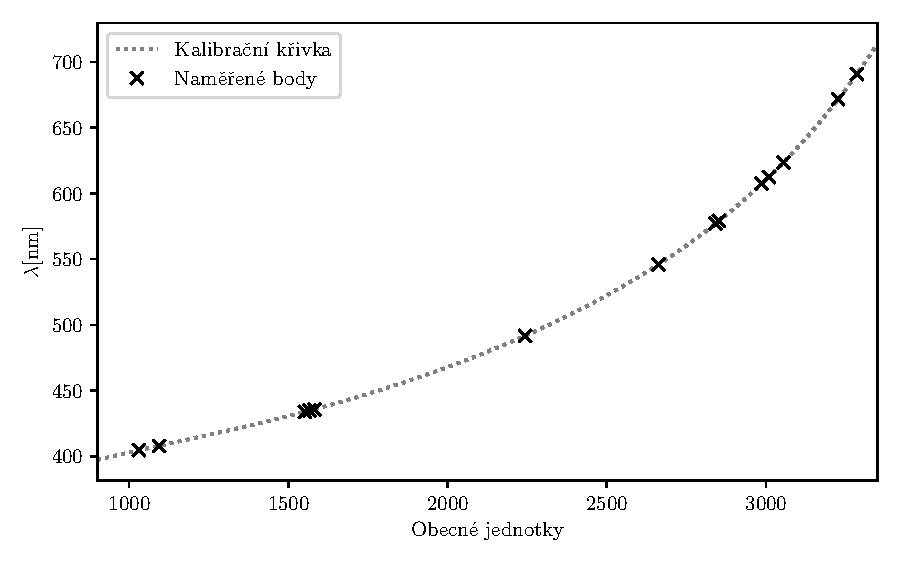
\includegraphics{plot.pdf}
        \caption{}
        \label{fig:fig}
    \end{figure}


    \section*{Diskuse}



    \section*{Závěr}



    \begin{thebibliography}{}

        \bibitem{pokyny}
        Pokyny k měření ``Studium atomových spekter'', dostupné z\\ \url{https://physics.mff.cuni.cz/vyuka/zfp/_media/zadani/texty/txt_415.pdf}, 12.\,11.\,2019

    \end{thebibliography}

\end{document}